\documentclass[../main]{subfiles}

\begin{document}

\begin{frame}{dangers of reductive algorithms}
\pnote{so last year I spoke about street-level algorithms, and how they look for and reinforce patterns of behavior, and how that bears on their propriety in novel situations or socially consequential contexts. but i didn't ask in that paper about how street-level algorithms cause us to change our behavior to ``present'' correctly to the algorithms}
\begin{center}
\visible<+->{``street-level algorithms'' struggle with novel situations}

\visible<+->{how are they changing \alert<2>{our lives} both offline and online?

\visible<+->{\dots and how \alert<3>{will} they?}}
\end{center}

\end{frame}




\begin{frame}

\pnote{and we're already seeing people pick up conspicuous behavior in direct response to algorithmic systems making the wrong calls. researchers like niloufar salehi and others have studied the use of ``finstas'', or fake instagram accounts allowing people to explore other aspects of their identities without instagram's recommendation algorithm putting that content in front of family. journalists have written about the collective use --- again of instagram --- accounts to confuse advertising and data collection algorithms. and in the wake of the COVID-19 pandemic, with YouTube demonetizing videos discussing COVID-19 (even in passing), youtubers have come up with coded language to avoid alerting the natural language processing system on the lookout for ``COVID-19''. in this example they call it the ``backstreet boys reunion tour''}

\vspace{2em}
\begin{columns}
\begin{column}{0.7\textwidth}{
  \begin{tikzpicture}[overlay]
      \visible<2->{\node[xshift=1cm] (img00)                 {\only<-4>{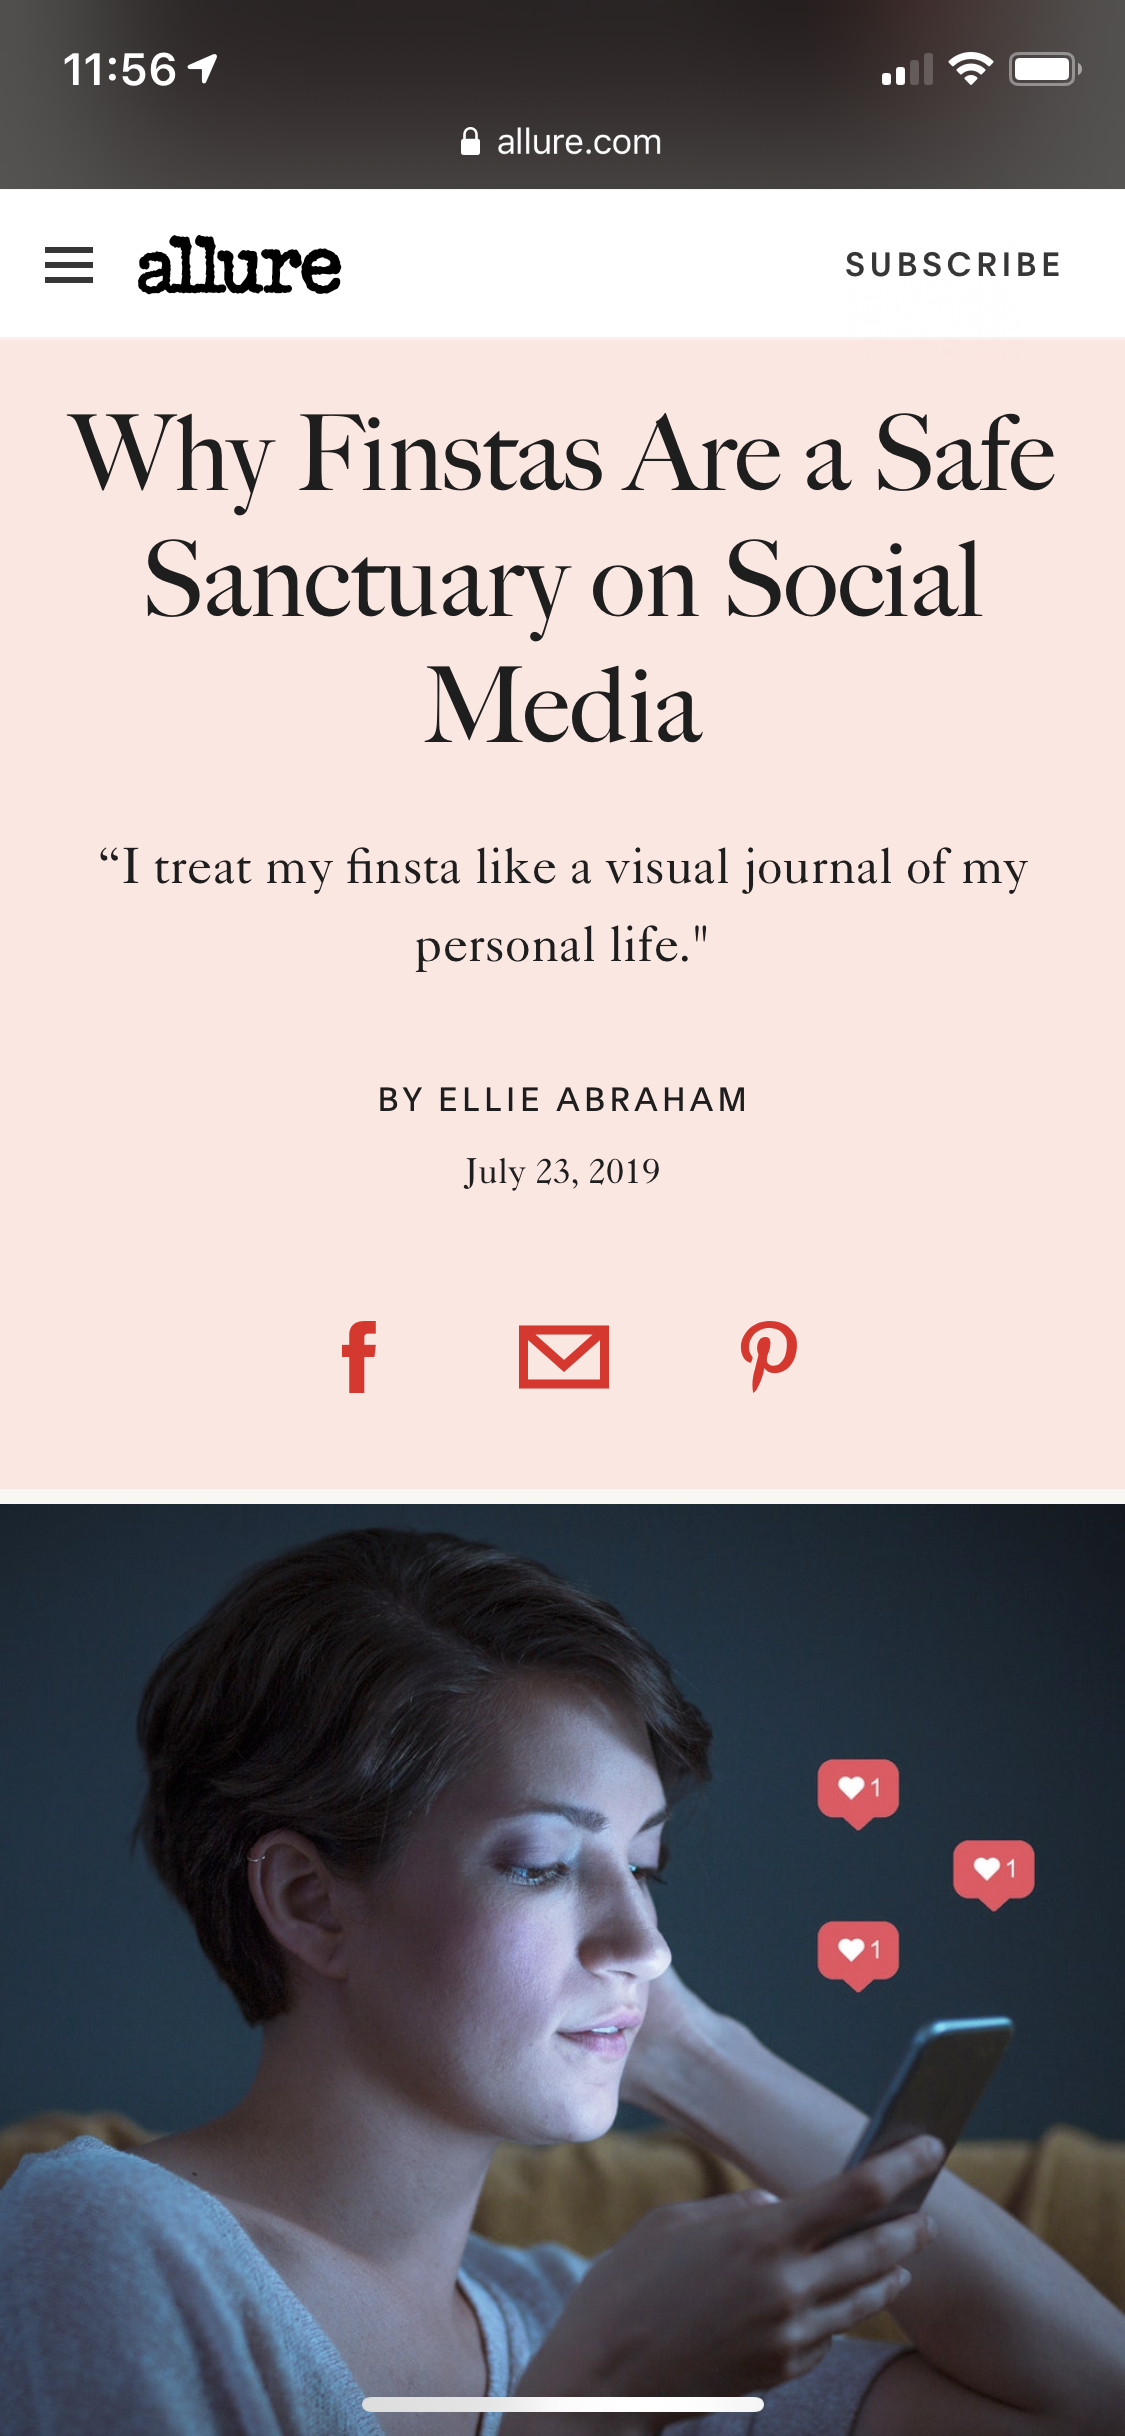
\includegraphics[width=0.4\textwidth]{../figures/algo_hiding/IMG_4828}}\only<5->{\includegraphics[width=0.4\textwidth]{../figures/algo_hiding/IMG_4828_grayed}}};}

      \visible<3->{\node [above right=-9cm and -0.5cm of img00] (img01) {\only<-4>{\includegraphics[width=0.4\textwidth]{../figures/algo_hiding/IMG_4830}}\only<5->{\includegraphics[width=0.4\textwidth]{../figures/algo_hiding/IMG_4830_grayed}}};}
      
      \visible<4->{\node [below right=-9cm and -0.5cm of img01] (img02) {\only<-4>{\includegraphics[width=0.4\textwidth]{../figures/algo_hiding/IMG_4832}}\only<5->{\includegraphics[width=0.4\textwidth]{../figures/algo_hiding/IMG_4832_grayed}}};}
  \end{tikzpicture}
  }
\only<6>{
\begin{center}
{\LARGE Digital Contact Tracing}
\end{center}
}
\end{column}
\end{columns}
\end{frame}

\end{document}
